\section{The AVR MCU Series}
\label{sec:atmega_overview}

	The Atmel AVR series is an enhanced-RISC MCU family that consists of the ATtiny, ATmega and ATxmega sub-categories and derivatives of the above, including 32-bit AVRs and application specific FPGAs\footnote{info:\href{http://www.atmel.com/products/microcontrollers/avr/default.aspx}{AVR family link}}. The models have varying degrees of hardware capabilities and large operating voltage windows in order to accommodate demand and integrate well with peripherals\footnote{info:\href{https://www.newbiehack.com/MicrocontrollersAlternativePowerSources.aspx}{https://www.newbiehack.com}}\footnote{info:\href{http://www.atmel.com/v2PFResults.aspx}{http://www.atmel.com/v2PFResults.aspx}}.
	
	Developing software for an AVR is easy as the AVRs benefit from the free \texttt{avr-libc} high-performance C run-time library(optimised for the AVR RISC architecture), the \texttt{avr-gcc} and \texttt{avr-gdb} compiler and debugger(both based on very popular and high quality GNU software tools), the \texttt{avrdude} programming software(or Atmel's proprietary \texttt{AVRStudio}) and \texttt{Simulavr} simulator software. Additionally, Atmel provides proprietary APIs for interacting with the AVR and the developers can choose from a wide variety of programmer units available for working with the AVRs\cite{book:practical_avr}.
	
	\subsection{ATMega Architecture and Features}				

	\subsubsection{Important Feature Overview}
	The ATmega series of MCUs is a relatively large family of MCUs and the focus of this paper is on the ATmega644 and ATmega1284. The only differences between then 1284 and the 644 is that the 1284 has got more memory available and an hardware extra timer. A summary of (some) of the features of the two units is give in Table \ref{table:avr_specs}\citep{atmega_manual}. 
	
	Both MCUs are an enhanced-RISC Harvard architecture 8-bit CPU. Figure \ref{fig:architectures} shows the conceptual difference between a Von Neuman (most modern PCs) and a Harvard architecture, where the key distinction lies in the separation of application code and program data into different memory sections (Harvard) and tasking the CPU with distinguishing between code and data that lives in the same memory region (Von Neuman). The 644/1284 implement a Harvard architecture for both power and computational efficiency, being designed to access more than one registers simultaneously (due to the physical wiring of the CPU), enabling them to execute an instruction per cycle. Their operating voltages can vary between 1.8V and 5.5V (maximum operating frequency 20 MHz).
	
	\subsubsection{Memory Organisation}
	The 644/1284 are equipped with an EEPROM, flash memory, SRAM, a large number of general purpose registers and a large number of I/O registers (in order to be able to perform I/O) and all memory (including I/O memory mapped images) is linear, i.e. it follows the flat memory model.
	
	The flash memory is separated into two regions, the bootloader section and application code section. The boundary between the two sections can be configured by programming the appropriate fuses, and the page size can also be configured that way as well. Both sections hold code, however code residing in the bootloader section can execute a special instruction (\texttt{SPM}\footnote{\texttt{SPM} = Store Program Code}) which allows the bootloader code to write to \textit{any} section in the flash memory and hence possibly modify itself(designed for purposes such as firmware upgrades). The bootloader code can be triggered by a direct jump from the application section or by programming the reset vector via the reset fuse to point to the appropriate section of the bootloader code. 
	
	The EEPROM is memory for data that needs to persist between reboots of the MCU and hence it is (widely) used to hold configuration variables and other non-temporary preferences the application code (or the bootloader) may need, having an average lifespan is 100,000 write cycles per page. 
	
	The SRAM is volatile storage and is used as the stack and heap for the software (either application code or bootloader code) as well as for storing the Register File (i.e. the 32 GP registers) I/O and Extended I/O Memory. The reserved register locations exist in order to support the use of peripheral units as well as hold program status information (e.g. the Stack Pointer can be found in one of the GP registers).Figure \ref{fig:stack} gives an overview of the SRAM hierarchy, which is slightly different (in terms of region sizes) for the 644 and the 1284 as the 1284 offers more SRAM.
	
	\begin{figure}
		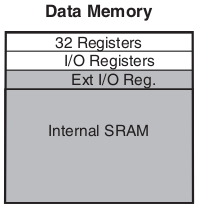
\includegraphics[scale=0.7]{img/stack.png}
		\caption{SRAM layout for the ATmega 644 and 1284. \textbf{Source}:\protect\citep{atmega_manual}.}
		\label{fig:stack}		
	\end{figure}
	
\begin{figure*}
	\begin{subfigure}{0.5\textwidth}
		\center
		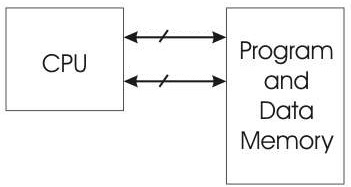
\includegraphics[scale=0.5]{img/von_neuman_arch.jpg}
		\caption{Schematic of a Von Neuman architecture.}
		\label{fig:VN_arch}
	\end{subfigure} 
	~
	\begin{subfigure}{0.5\textwidth}
		\center
		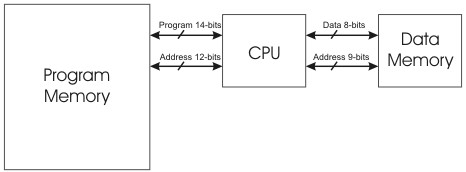
\includegraphics[scale=0.5]{img/harvard_arch.jpeg}
		\caption{Schematic of a Harvard architecture.}
		\label{fig:H_arch}
	\end{subfigure}
	\caption{A comparison of different machine architectures. \textbf{Source}:\protect\citep{website:mcu_primer}.}
	\label{fig:architectures}
\end{figure*}	
		
\begin{table}
	\begin{tabular}{| c | p{2cm} | p{1.5cm} | p{1.5cm} | p{2.8cm} | p{1.9cm} |}
		\textbf{Model} & \textbf{EEPROM (Kb)} & \textbf{SRAM (Kb)} & \textbf{Flash (Kb)}\\
		ATmega644 & 2 & 4 & 64\\
		ATmega1284 & 4 & 16 & 128\\
	\end{tabular}
	\caption{Specification overview for the AVR ATmega644 and ATmega1284}
	\label{table:avr_specs}
\end{table}
	
	\subsection{ATMega Security Features}
	
	The AVR ATmega644/1284, even though not meant to be secure hardware modules, posses certain security features. In particular, each board provides six Lock bits responsible for controlling access to the board's memory and prevent reading or modifying the memory (e.g. prevent code executing from the bootloader section to read/write the application code section via the \texttt{SPM} instruction). This access control is not permanent, as that would limit the usefulness of the MCU and therefore one has the option to reset the lock bits (i.e. having no protection scheme enabled) by issuing a Chip Erase command, which has the effect of completely erasing the Flash, EEPROM and Lock bits.
	
	The erasing is performed with the sequence of events presented above and this is important, as one does not want to remove the access protection before removing all sensitive data and hence the Lock bits are set to 1 only after the whole program memory has been erased. Even though the flash memory has an average lifespan of 10,000 write cycles (as well as programming being relatively expensive as an operation) this approach makes sense as the ultimate goal is to preserve the intellectual property on the board rather than the board itself.
	
	\begin{table}
		\center
		\begin{tabular}{| c | c | c | c |}
			\hline
			\textbf{Lock Bit Byte} & \textbf{Bit Number} & \textbf{Default}\\
			\hline \hline
			BLB12 & 5 & 1\\
			BLB11 & 4 & 1\\
			BLB02 & 3 & 1\\
			BLB01 & 2 & 1\\
			LB2 & 2 & 1 \\
			LB1 & 1 & 1 \\
			\hline
		\end{tabular}
		\caption{Security lock bits offered by the ATmega644 and ATmega1284. BLB stands for Boot Lock Bit and LB for Lock Bit.}
		\label{table:lock_bits}
	\end{table}
	
Table \ref{table:lock_bits}	 provides an outline of the available Lock bits provided by the ATmega series. The functionality of the BLB1 group is to control access and modification of the bootloader section, group BLB0 bits control access to the application code section and group LB bits are responsible for controlling modifications on the EEPROM and Flash.A detailed explanation of their functionality and how to use them is given in \citep{atmega_manual}.
	